\section{Projeto de observador}

\subsection{Identificação de sistemas}

Considerando a equação da função de transferência padrão \ref{z:default}, a sua equação diferença será na forma:

\begin{center}
    $y[n+2] = cx[n+1] + dx[n] + ay[n+1] - by[n]$\vspace{4pt}\\
\end{center}

Assim, um modelo básico para identificação dos coeficientes do sistema podem ser considerados pela equação matricial \ref{id:default} para um conjunto de $N$ amostras:

\begin{equation} \label{id:default}
\centering
\begin{bmatrix} y[2] \\ y[1] \\ \vdots \\ y[N] \end{bmatrix} = \begin{bmatrix} u[1] & u[0] & -y[1] & -y[0] \\ u[2] & u[1] & -y[2] & -y[1] \\ \vdots & \vdots & \vdots & \vdots \\ u[N-1] & u[N-2] & -y[N-1] & -y[N-2]\end{bmatrix}\begin{bmatrix} c \\ d \\ a \\ b \end{bmatrix}
\end{equation}

Com $y$ representando o vetor de amostras da resposta do sistema analógico e $u$ a entrada do sistema. Para uma identificação mais precisa do sistema, a entrada deve possuir componentes frequenciais que busquem explorar todos os modos de excitação do sistema.

O sistema acima pode ser escrito como a equação matricial: $y = Mc$, de forma que o vetor de coeficientes pode ser encontrado por: $c = M^{-1}y$. Porém, como a matriz M não é quadrada, ela não possuirá inversa, sendo necessário recorrer à pseudo inversa: 

\begin{equation} \label{id:matriz}
c = (M^tM)^{-1}M^t v 
\end{equation}

\subsubsection{Sistema estável}

Para a identificação do sistema estável, foi utilizada uma entrada de pulsos de amplitudes aleatórias (variam de 0 a 1) com no mínimo uma frequência de amostragem de 100 vezes maior que a do sistema simulado, gerando uma saída do sistema contínuo simulado no XCOS do Scilab. Essa saída foi utilizada para computar o vetor de coeficientes de acordo com a equação matricial \ref{id:matriz}.

O perfil da entrada utilizada comparada com a saída encontrada estão apresentados na figura \ref{id:est:entsai}

\begin{figure}[H]
\begin{center}
    \subfigure[Entrada]{             
        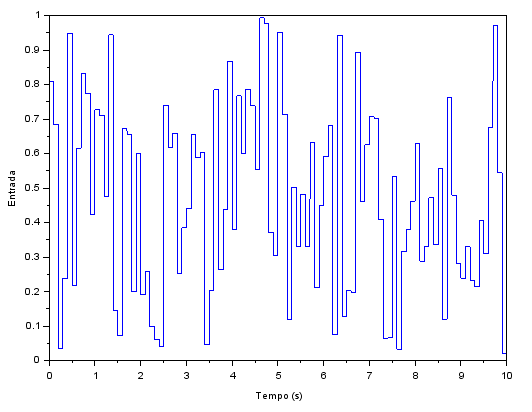
\includegraphics[width=7.5cm]{images/id/random_est_1e-1.png}  
        \label{id:est:entsai:1}
    }
    \subfigure[Saída]{                                              
        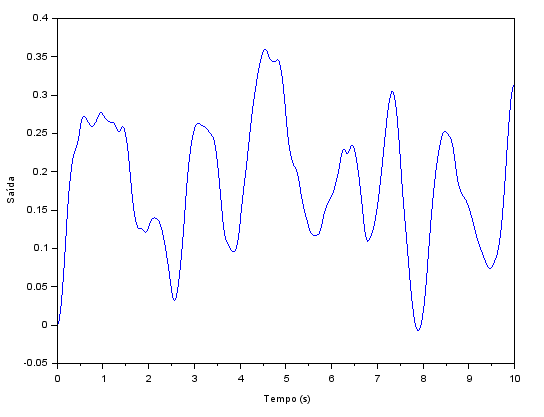
\includegraphics[width=7.5cm]{images/id/output_est_1e-1.png}
        \label{id:est:entsai:2}
    }                
\end{center}
\caption{(a) Entrada aleatória e sua respectiva (b) saída para o sistema estável.}
\label{id:est:entsai} 
\end{figure}

Utilizando o vetor saída encontrado no passo anterior para identificar o sistema, observou-se que o vetor de coeficientes encontrados foi:

\begin{itemize}
    \item $a = 1.9768486$;
    \item $b = 0.9792891$;
    \item $c = 0.0008145$;
    \item $d = 0.0001605$;
\end{itemize}

Comparando com os coeficientes originais:

\begin{itemize}
    \item $a = 1.977724$;
    \item $b = 0.9801987$
    \item $c = 0.0004966$
    \item $d = 0.0004933$
\end{itemize}

Pela comparação observa-se que os coeficientes do denominador possuem uma alta correspondência, enquanto que, à primeira vista, os coeficientes do numerador diferem. Essa falta de correspondência é solucionada ao simular o sistema para uma entrada degrau unitário, resultando na figura \ref{id:est:corr}.

\begin{figure}[H]
\begin{center}
    \subfigure[Saídas]{             
        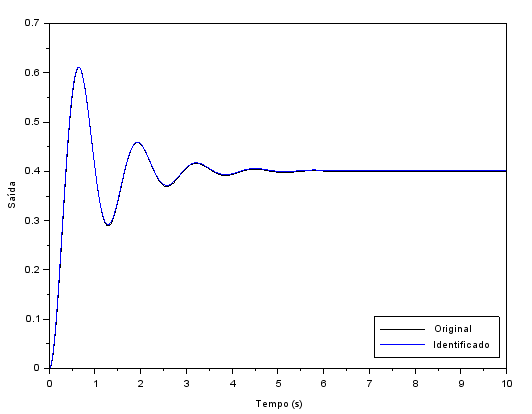
\includegraphics[width=7.5cm]{images/id/output_comp_est.png}  
        \label{id:est:corr:1}
    }
    \subfigure[Comparação]{                                              
        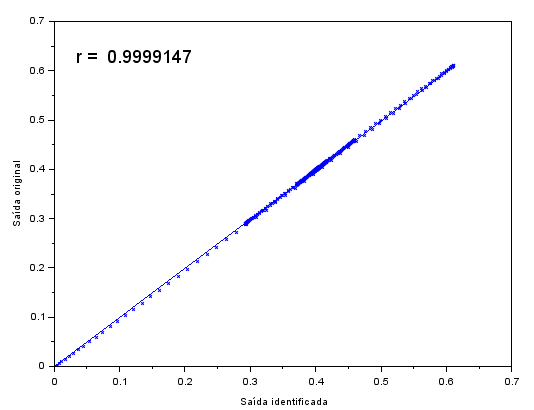
\includegraphics[width=7.5cm]{images/id/corr_comp_est.png}
        \label{id:est:corr:2}
    }                
\end{center}
\caption{(a) Comparação entre as saídas para os sistemas original e identificado e a (b) correlação dos valores.}
\label{id:est:corr} 
\end{figure}

De acordo com a figura, observa-se que a comparação da resposta do sistema identificado com o sistema discreto simulado com os coeficientes originais possuem uma alta correlação, representando um bom modelo para identificação de sistemas contínuos. Porém, deve ser levado em conta que o sistema identificado é tão preciso quanto diversificado for o sinal de entrada.

\subsubsection{Sistema instável}

A identificação do sistema instável é um pouco mais difícil, pois entradas que possuem um \textit{offset} levam o sistema a um crescimento indefinido. Neste caso o sistema instabilizando, seus modos de excitação não são amplamente explorados, resultando em coeficientes que equivalem a um sistema que diverge significativamente, ou uma matriz singular.

A alternativa encontrada foi realizar a realimentação negativa de ganho unitário na planta para que ela se estabilize. Considerando que a planta em malha aberta é aquela da equação \ref{z:ins}, tem-se que a planta em malha fechada a partir do mesmo processo de discretização submetido anteriormente (processo facilitado pela função \textit{c2d} do MATLAB), será:

\begin{equation} \label{z:ins:MF}
    H_{ins}(z) = \frac{0.009819 z + 0.009657}{z^2 - 1.932 z + 0.9512}
\end{equation}

Observa-se nessa planta que o numerador continua o mesmo que o da malha aberta e que os coeficientes do denominador mudaram de acordo com o numerador (número pequeno, o suficiente para que o sistema não instabilize. Desta forma ao realizar a identificação para esse sistema, basta subtrair os coeficientes encontrados para o numerador dos devidos coeficientes do numerador.

Outro detalhe importante é que a matriz do sistema \ref{id:default} irá mudar. Uma vez que a entrada $u$ não mais representará a entrada global do sistema, mas apenas o erro. 

A partir deste ponto, a análise é análoga à anterior. O perfil da entrada utilizada comparada com a saída encontrada estão apresentados na figura \ref{id:ins:entsai}. Neste caso, foi optado por uma entrada mais simples, mas ainda gerada randomicamente.

\begin{figure}[H]
\begin{center}
    \subfigure[Entrada]{             
        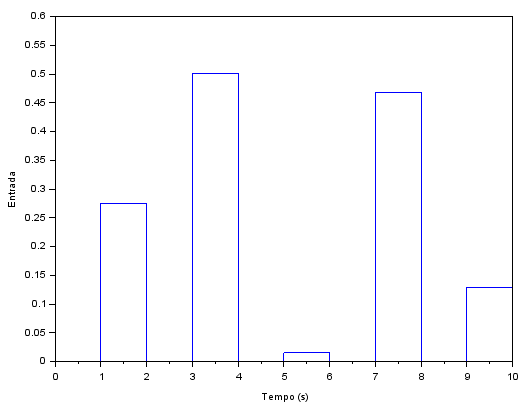
\includegraphics[width=7.5cm]{images/id/random_ins_1e-0.png}  
        \label{id:ins:entsai:1}
    }
    \subfigure[Saída]{                                              
        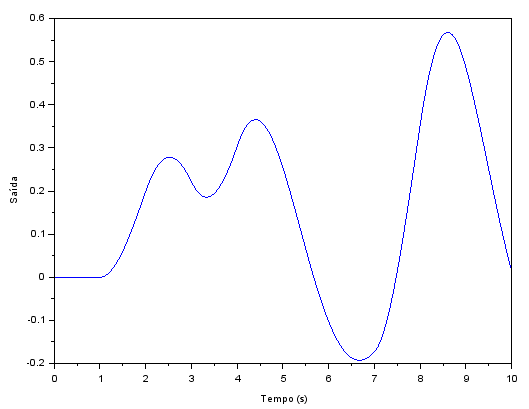
\includegraphics[width=7.5cm]{images/id/output_ins_1e-0.png}
        \label{id:ins:entsai:2}
    }                
\end{center}
\caption{(a) Entrada aleatória e sua respectiva (b) saída para o sistema instável.}
\label{id:ins:entsai} 
\end{figure}

Utilizando o vetor saída encontrado no passo anterior para identificar o sistema, observou-se que o vetor de coeficientes encontrados foi:

\begin{itemize}
    \item $a = 1.9994965$;
    \item $b = 0.9994965$;
    \item $c = 0.0000024$;
    \item $d = -0.0000004$;
\end{itemize}

Comparando com os coeficientes originais:

\begin{itemize}
    \item $a = 1.9512294$;
    \item $b = 0.9512294$
    \item $c = 0.0098354$
    \item $d = 0.00967728$
\end{itemize}

Pela comparação observa-se que os coeficientes do denominador possuem uma relativa correspondência, enquanto que, à primeira vista, os coeficientes do numerador diferem. Essa falta de correspondência é solucionada ao simular o sistema para uma entrada degrau unitário e com período de amostragem adequado à corresponder, resultando na figura \ref{id:est:corr} que permite concluir que a representação foi boa.

\begin{figure}[H]
\begin{center}
    \subfigure[Saídas]{             
        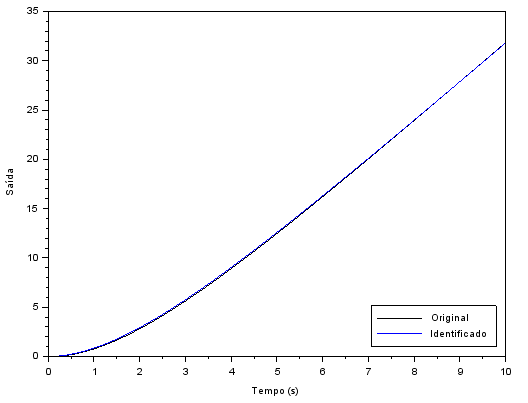
\includegraphics[width=7.5cm]{images/id/output_comp_ins.png}  
        \label{id:ins:corr:1}
    }
    \subfigure[Comparação]{                                              
        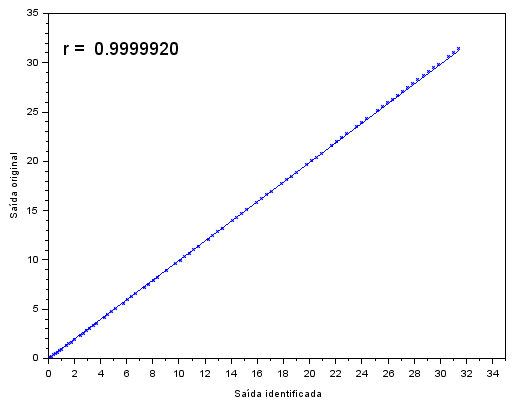
\includegraphics[width=7.5cm]{images/id/corr_comp_ins.png}
        \label{id:ins:corr:2}
    }                
\end{center}
\caption{(a) Comparação entre as saídas para os sistemas original e identificado e a (b) correlação dos valores.}
\label{id:ins:corr} 
\end{figure}


\subsection{Análise de controlabilidade e observabilidade em tempo discreto}

Será verificada a controlabilidade e observabilidade de cada uma das plantas a partir das representações em espaço de estados em tempo discreto. Em seguida, para cada análise, a planta será reescrita na forma canônica controlável ou observável.

Um sistema linear invariante no tempo será controlável se e somente se, a matriz de controlabilidade da equação \ref{controlabilidade} de dimensões $n \times m.s$ possuir posto $n$. Enquanto que para ser observável, a matriz de observabilidade da equação \ref{observabilidade} de dimensões $l.n \times n$ deve possuir posto $n$.

\begin{equation} \label{controlabilidade}
    W_C = \begin{bmatrix} \Gamma & \Phi \Gamma \end{bmatrix}
\end{equation}
\begin{equation} \label{observabilidade}
    W_O = \begin{bmatrix} C \\ C \Phi \end{bmatrix}
\end{equation}

A partir da representação em FADALI (2013), a representação na forma canônica controlável e observável do sistema padrão adotado neste trabalho por meio da equação \ref{z:default} são representadas, respectivamente, pelos sistemas de equações \ref{ctrl:canon} e \ref{obsv:canon}.

\begin{equation} \label{ctrl:canon}
\centering
\left \{
\begin{array}{cc}
x[n+1] = \begin{bmatrix} 0 & 1 \\ -b & a \end{bmatrix} x[n] + \begin{bmatrix} 0 \\ 1 \end{bmatrix} u[n] \\
y[n] = \begin{bmatrix} d & c  \end{bmatrix} x[n] \\
\end{array}
\right.
\end{equation}

\begin{equation} \label{obsv:canon}
\centering
\left \{
\begin{array}{cc}
x[n+1] = \begin{bmatrix} a & 1 \\ -b & 0 \end{bmatrix} x[n] + \begin{bmatrix} c \\ d \end{bmatrix} u[n] \\
y[n] = \begin{bmatrix} 1 & 0  \end{bmatrix} x[n] \\
\end{array}
\right.
\end{equation}

\subsubsection{Controlabilidade e forma canônica controlável}

Considerando o sistema estável, sua matriz de controlabilidade será:

\begin{equation} \label{ctrl:1}
    W_{C_{EST}} = \begin{bmatrix}  0.0004966 & 0.0014754\\ 0.0989654 & 0.0967608\end{bmatrix}
\end{equation}

Enquanto que para o sistema instável, sua matriz de controlabilidade será:

\begin{equation} \label{ctrl:2}
    W_{C_{INS}} = \begin{bmatrix}  0.0098354 & 0.0288639\\ 0.1950823 & 0.185568\end{bmatrix}
\end{equation}

Dessa forma, observando que todas as linhas da matriz de controlabilidade da planta estável e instável são linearmente independentes, com posto 2 (ou o determinante não nulo), logo os sistemas nessa representação são controláveis.

Caso a representação em espaço de estados considerada até agora não fosse controlável, uma solução seria representar o sistema em sua forma canônica controlável a partir da função de transferência discreta que garante que ele seja sempre controlável. Assim, a partir da fórmula expressa na equação \ref{ctrl:canon} a partir da literatura e para um sistema de ordem 2, a representação na forma canônica controlável para o sistema estável e instável podem ser observadas nos sistemas \ref{ctrl:canon:est} e \ref{ctrl:canon:ins}, respectivamente.


\begin{equation} \label{ctrl:canon:est}
\centering
\left \{
\begin{array}{cc}
x[n+1] = \begin{bmatrix} 0 & 1 \\ -0.9801987 & 1.977724 \end{bmatrix} x[n] + \begin{bmatrix} 0 \\ 1 \end{bmatrix} u[n] \\
y[n] = \begin{bmatrix} 0.0004933 & 0.0004966  \end{bmatrix} x[n] \\
\end{array}
\right.
\end{equation}

\begin{equation} \label{ctrl:canon:ins}
\centering
\left \{
\begin{array}{cc}
x[n+1] = \begin{bmatrix} 0 & 1 \\ -0.9512294 & 1.9512294 \end{bmatrix} x[n] + \begin{bmatrix} 0 \\ 1 \end{bmatrix} u[n] \\
y[n] = \begin{bmatrix} 0.00967728 & 0.0098354  \end{bmatrix} x[n] \\
\end{array}
\right.
\end{equation}

\subsubsection{Observabilidade e forma canônica observável}

Considerando o sistema estável, sua matriz de observabilidade será:

\begin{equation} \label{obsv:1}
    W_{O_{EST}} = \begin{bmatrix}  1 & 0\\ 0.9987586 & 0.0098965\end{bmatrix}
\end{equation}

Enquanto que para o sistema instável, sua matriz de observabilidade será:

\begin{equation} \label{obsv:2}
    W_{O_{INS}} = \begin{bmatrix}  1 & 0\\ 1 & 0.0975412\end{bmatrix}
\end{equation}

Dessa forma, observando que todas as linhas da matriz de observabilidade da planta estável e instável são linearmente independentes, com posto 2 (ou o determinante não nulo), logo os sistemas nessa representação são observáveis.

De acordo com o que foi discutido para a forma canônica controlável, também é aplicável a transformação do sistema para sua forma canônica observável, garantindo a observabilidade. Assim, a partir da fórmula expressa na equação \ref{obsv:canon} a partir da literatura e para um sistema de ordem 2, a representação na forma canônica observável para o sistema estável e instável podem ser observadas nos sistemas \ref{obsv:canon:est} e \ref{obsv:canon:ins}, respectivamente.

\begin{equation} \label{obsv:canon:est}
\centering
\left \{
\begin{array}{cc}
x[n+1] = \begin{bmatrix} 1.977724 & 1 \\ -0.9801987 & 0 \end{bmatrix} x[n] + \begin{bmatrix} 0.0004966 \\ 0.0004933 \end{bmatrix} u[n] \\
y[n] = \begin{bmatrix} 1 & 0  \end{bmatrix} x[n] \\
\end{array}
\right.
\end{equation}

\begin{equation} \label{obsv:canon:ins}
\centering
\left \{
\begin{array}{cc}
x[n+1] = \begin{bmatrix} 1.9512294 & 1 \\ -0.9512294 & 0 \end{bmatrix} x[n] + \begin{bmatrix} 0.0098354 \\ 0.00967728 \end{bmatrix} u[n] \\
y[n] = \begin{bmatrix} 1 & 0  \end{bmatrix} x[n] \\
\end{array}
\right.
\end{equation}


\subsection{Observadores de estado}

Os observadores de estado projetados partiram da equação \ref{tran:2} para obter os polos do observador que são encontrados na forma: $a^*(z) = z^2 - (\lambda_1+\lambda_2) + (\lambda_1+\lambda_2)$. Assim, escolhe-se os polos para $\omega_n = 3.384 rad/s$ e $\xi = 0.591$, obtendo $\lambda_1=0.979916$ e $\lambda_2=0.980481$, para os polos do observador do sistema estável e $\lambda_{1,2}=0.818726\pm j0.00278153$, para os polos do observador do sistema instável.

A partir dos polos encontra-se a matriz L de ganhos do observador. Resolvendo o sistema de equações $det(\lambda I - \Phi - LC) = 0$ para os polos do observador, permite-se encontrar a matriz L. O sistema foi considerado aquele na forma canônica observável que garante que o sistema sempre será observável. Para ambos os sistemas, a matriz encontrada foi:

\begin{center}
$L_{est} = \begin{bmatrix} 0.017327 \\ -0.0194097 \end{bmatrix}$; $L_{ist} = \begin{bmatrix} 0.3137774 \\ -0.2809094 \end{bmatrix}$
\end{center}

A partir das matrizes encontradas, foi realizada a simulação do sistema com o observador de estado em malha fechada (equação matricial \ref{obs:eq}) para observar como as variáveis de estado estimadas se comportam em relação às variáveis originais.

\begin{equation} \label{obs:eq}
\centering
\left \{
\begin{array}{cc}
\tilde{x}[n+1] = (\Phi-LC) \tilde{x}[n] + \Gamma u[n] + L y[k] \\
\tilde{y}[n] = C \tilde{x}[n] + D u[n]\\
\end{array}
\right.
\end{equation}

Antes de realizar a simulação, os valores de saída originais foram somados a um sinal aleatório limitado em $\pm 0.05$ para funcionar como ruído.

Dessa forma, foram avaliadas como as variáveis de estado estimadas se comportam e seus erros relativos às variáveis originais. O erro será avaliado com e sem adição de ruído. 


\begin{figure}[H]
\begin{center}
    \subfigure[$x_1$]{             
        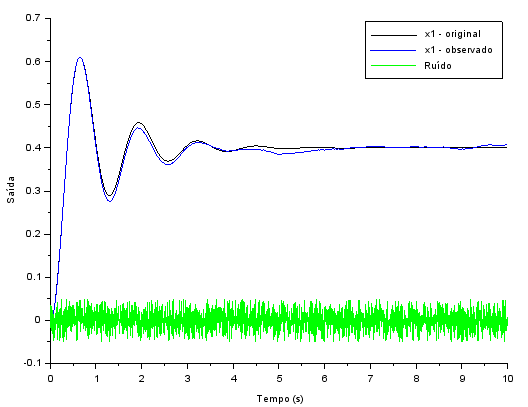
\includegraphics[width=7.5cm]{images/obs/est_x1.png}  
        \label{obs:est:x:1}
    }
    \subfigure[$x_2$]{                                              
        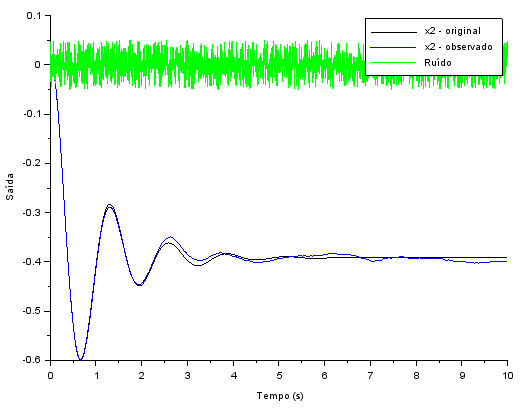
\includegraphics[width=7.5cm]{images/obs/est_x2.png}
        \label{obs:est:x:2}
    }                
\end{center}
\caption{Comparação entre as variáveis de estado estimadas e originais (a) 1 e (b) 2, do sistema estável.}
\label{obs:est:x} 
\end{figure}

\begin{figure}[H]
\begin{center}
    \subfigure[Com ruído]{             
        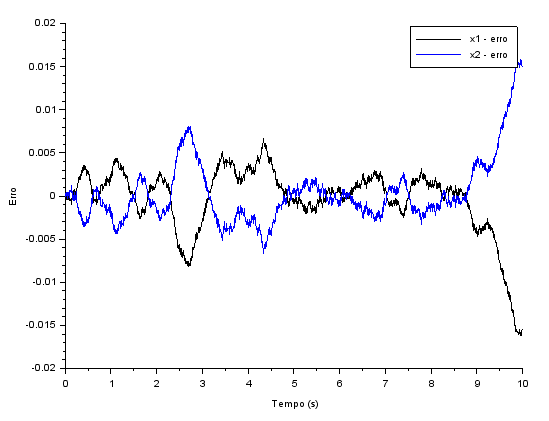
\includegraphics[width=7.5cm]{images/obs/est_erro.png}  
        \label{obs:est:err:1}
    }
    \subfigure[Sem ruído]{                                              
        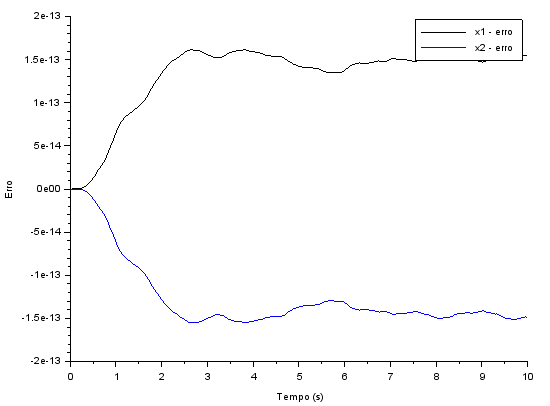
\includegraphics[width=7.5cm]{images/obs/est_erro_nornd.png}
        \label{obs:est:err:2}
    }                
\end{center}
\caption{Comparação entre os erros entre as variáveis de estados, considerado o caso em que (a) um sinal de erro é somado à saída original do sistema estável e (b) quando não é.}
\label{obs:est:err} 
\end{figure}

\begin{figure}[H]
\begin{center}
    \subfigure[$x_1$]{             
        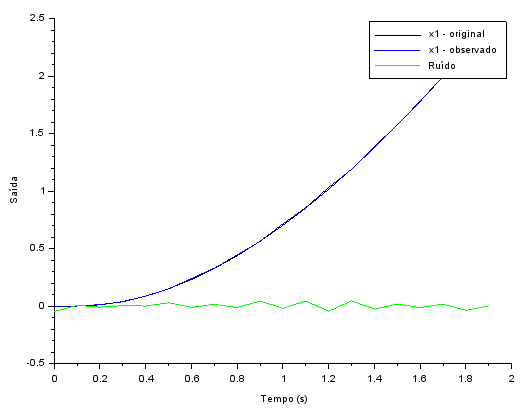
\includegraphics[width=7.5cm]{images/obs/ins_x1.png}  
        \label{obs:ins:x:1}
    }
    \subfigure[$x_2$]{                                              
        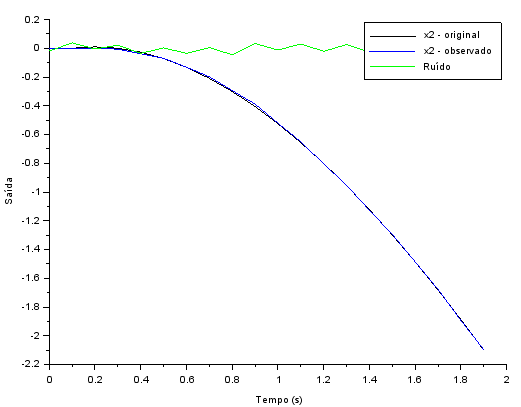
\includegraphics[width=7.5cm]{images/obs/ins_x2.png}
        \label{obs:ins:x:2}
    }                
\end{center}
\caption{Comparação entre as variáveis de estado estimadas e originais (a) 1 e (b) 2, do sistema instável.}
\label{obs:ins:x} 
\end{figure}

\begin{figure}[H]
\begin{center}
    \subfigure[Com ruído]{             
        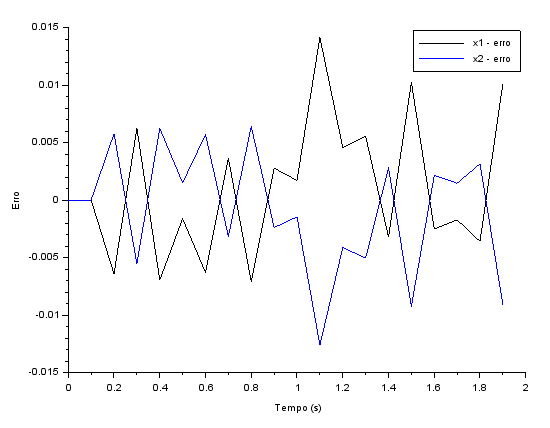
\includegraphics[width=7.5cm]{images/obs/ins_erro.png}  
        \label{obs:ins:err:1}
    }
    \subfigure[Sem ruído]{                                              
        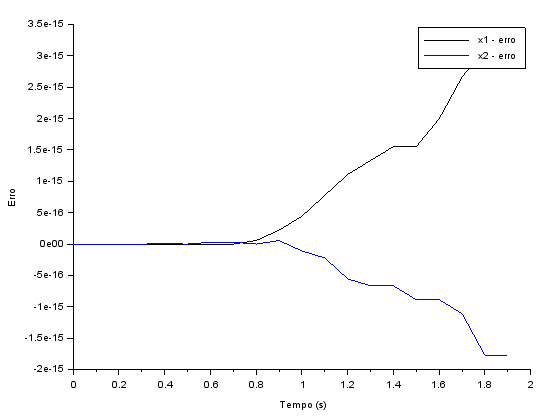
\includegraphics[width=7.5cm]{images/obs/ins_erro_nornd.png}
        \label{obs:ins:err:2}
    }                
\end{center}
\caption{Comparação entre os erros entre as variáveis de estados, considerado o caso em que (a) um sinal de erro é somado à saída original do sistema instável e (b) quando não é.}
\label{obs:ins:err} 
\end{figure}

A partir dos resultados, pode-se notar que o observador de estados possui uma alta fidelidade em estimar os estados reais do sistema. Porém, de acordo com os resultados para o sistemas estável, notou-se um ligeiro aumento no erro de acordo com que o sinal alcançava a região de regime, enquanto que na planta instável esse efeito é inexistente. Outro fato a ser analisado é o comportamento do erro de acordo com a presença do ruído, mudando significativamente o erro e o tornando imprevisível. Há de notar que, principalmente no caso estável que possui uma maior frequência de amostragem, o ruído, que possui alta frequências, foi modulado pelo erro.

Ao atribuir polos mais rápidos para o observador, observou que, de fato, o erro se propagava com maior intensidade, exaltando a importância de que um bom projeto de observador, na prática, faz toda a diferença.

\pagebreak